% !TeX root = ../economia.tex
\chapter{Organizzazione aziendale}

% Increase vertical spacing of tables
\def\arraystretch{1.5}

\section{Impresa come sistema complesso e aperto}

L'impresa può essere vista come \emph{sistema complesso}, ovvero un \emph{insieme di parti interagenti fra loro}.

In particolare l’impresa è contraddistinta da:
\begin{itemize}
	\item presenza di un numero elevato di \emph{compiti} che necessitano di essere \emph{coordinati} tra loro
	\item insieme di \emph{persone}: la conseguenza delle azioni
	sulle persone non sono del tutto prevedibili
\end{itemize}

L’impresa è un sistema aperto, ovvero in continua interazione
con l’ambiente (e non solo
con le sue componenti interne), e per questo motivo
deve essere inserita in un contesto più ampio, in cui è influenzata da un insieme di fattori che non
risultano del tutto prevedibili e/o controllabili, gli \emph{stakeholders}:
\begin{itemize}
	\item concorrenti
	\item fornitori/clienti
	\item stato/istituzioni
	\item sistema finanziario
\end{itemize}

\begin{figure}[h]
	\centering
	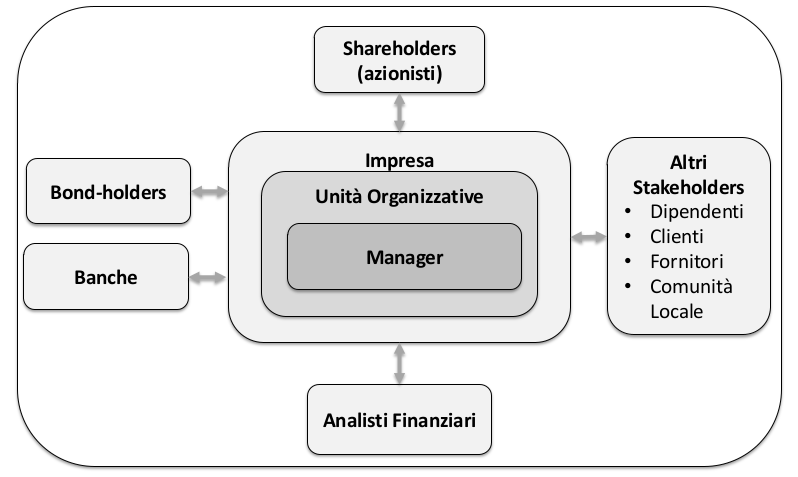
\includegraphics[width=0.5\linewidth]{images/azienda_sistema_aperto}
	\caption[Azienda vista come sistema aperto]{}
	\label{fig:aziendasistemaaperto}
\end{figure}

L’impresa è un sistema aperto \emph{orientato alla creazione di valore
economico}.
L’\emph{obiettivo primario} di un’impresa è rappresentato in primo luogo
dalla creazione di \emph{valore economico} per i propri azionisti:

\[
V(0) = \sum_{t=0}^\infty \frac{FF(t)}{(1+k)^t}
\]

dove $V(0)$ è il valore economico, $FF(t)$ sono i flussi di cassa netti annui dall’impresa verso gli
azionisti e $k$ è il tasso opportunità annuo.

Poiché l’ambiente è in continua evoluzione non si ha un
equilibrio, ma eventualmente uno \emph{stato stazionario}.

Se l’ambiente si modifica l’impresa deve reagire attraverso un
adattamento per poter sopravvivere.
In particolare le imprese possono pianificare
e realizzare cambiamenti che vanno a modificare:
\begin{itemize}
	\item le relazioni con l’ambiente
	\item la struttura interna
e le	attività operative dell’organizzazione
\end{itemize}

Da un punto di vista interno l’impresa può essere concepita
come un insieme di insiemi organizzati secondo una
gerarchia di obiettivi:
\begin{itemize}
	\item gli elementi sono a loro volta dei sistemi decomponibili
	\item ogni elemento deve essere interconnesso con almeno un altro secondo una legge specifica
	\item gli obiettivi di un sottosistema dipendono in maniera
	gerarchica dagli obiettivi del sovrasistema
\end{itemize}

\section{L'organizzazione aziendale}
L'organizzazione può essere definita come il
complesso delle modalità secondo le quali
viene effettuata la \emph{divisione del lavoro} in
compiti distinti e quindi realizzato il
\emph{coordinamento} tra tali compiti.

\vspace{1em}
\begin{tabular}{|c|c|c|}
	\cline{2-3}
 	\multicolumn{1}{c|}{} & Microstruttura & Macrostruttura \\
	\hline
	Divisione del lavoro & Specializzazione & Criteri di raggruppamento \\
	\hline
	Coordinamento & \multicolumn{2}{c|}{Meccanismi di coordinamento} \\
	\hline\hline
	Formalizzazione & Mansionari & Organigramma \\
	\hline
\end{tabular}

\subsection{Definizioni}

\paragraph{Microstruttura (o posizione individuale)} insieme di mansioni e ruoli assegnabili ad un'unica persona.

\paragraph{Mansione} insieme dei compiti elementari assegnabili ad una
posizione aziendale che può essere ricoperta da una persona.

\paragraph{Compito} insieme di attività o operazioni necessariamente collegate
in funzione di proprietà/capacità del lavoro umano e
tecnica impiegata.

\paragraph{Specializzazione orizzontale}

Numero di compiti diversi attribuibili ad ogni mansione per
raggiungere un determinato output.
Può essere \emph{alta} (una persona svolge un compito specialistico) o \emph{bassa} (una persona svolge
più compiti).

\paragraph{Specializzazione verticale}
La separazione tra le attività \emph{esecutive} e quelle di
\emph{programmazione e controllo}.
Indica, quindi, il livello di profondità della mansione. Può essere \emph{alta} (una persona non decide
ma si limita ad eseguire, come un operaio) o \emph{bassa} (una persona
prevalentemente decide, come un manager).


\subsection{Legami tra specializzazione orizzontale e verticale}
Di solito c'è una correlazione \emph{diretta} tra specializzazione orizzontale e verticale:
un'alta specializzazione orizzontale
corrisponde ad un'alta specializzazione verticale.

\begin{table}[h]
	\begin{tabular}{cc|c|c|}
		\cline{3-4}
		&       & \multicolumn{2}{c|}{Specializzazione orizzontale}  \\ \cline{3-4} 
		&       & Alta                     & Bassa                   \\ \hline
		\multicolumn{1}{|c|}{\multirow{2}{*}{Specializzazione verticale}} & Alta  & Mansioni non qualificate & Mansioni professionali  \\ \cline{2-4} 
		\multicolumn{1}{|c|}{}                                            & Bassa & Manager di basso livello & Manager di alto livello \\ \hline
	\end{tabular}
\end{table}
\begin{itemize}
	\item \emph{Alta specializzazione orizzontale} e \emph{alta specializzazione verticale}:
	è questa l’ipotesi che si risconta nel caso di lavori poco qualificati
	(esempio: operai che svolgono compiti molto elementari)
	
	\item \emph{Alta specializzazione orizzontale} e \emph{bassa specializzazione
	verticale}: è il caso del lavoro direzionale svolto ai livelli più bassi della
	struttura aziendale. Si tratta di
	lavoro che richiede lo svolgimento di una pluralità di compiti di
	controllo, coordinamento, direzione, ma soggetti ad un controllo
	piuttosto rigido
	\item \emph{Bassa specializzazione orizzontale} e \emph{alta specializzazione
	verticale}: è il caso del lavoro direzionale svolto ai livelli più bassi della
	struttura aziendale. È la situazione nella quale si trovano quegli
	organi che svolgono pochi compiti e sono dotati di grossa autonomia
	\item \emph{Bassa specializzazione orizzontale} e \emph{bassa specializzazione
	verticale}: è il caso del lavoro svolto dai manager e dai dirigenti di alto
	livello che devono essere poco specializzati in quanto devono avere
	una visione d’insieme, ma godono del più ampio potere decisionale.
\end{itemize}

\subsection{Meccanismi di coordinamento}
\paragraph{Adattamento reciproco (mutuo adattamento)}
coordinamento tramite il semplice processo di comunicazione informale.

\paragraph{Supervisione diretta}
prevede la presenza di un individuo che si assume la responsabilità del
lavoro di altri, dando loro ordini e controllando le loro azioni.
\paragraph{Standardizzazione delle competenze}
consiste nello specificare il tipo di formazione e competenze richieste per
eseguire un determinato lavoro e selezionare le persone di
conseguenza.
\paragraph{Standardizzazione dei processi}
consiste nello specificare o programmare in modo dettagliato i contenuti
del lavoro.
\paragraph{Standardizzazione degli output} si basa sulla determinazione e valutazione dei risultati del lavoro.

\paragraph{Formalizzazione del comportamento}
Modo in cui l'impresa elimina la discrezionalità dei suoi dipendenti e
delle sue unità organizzative, essenzialmente descrivendo
minuziosamente regole, procedure, ruoli e responsabilità.
Lo strumento per formalizzare il comportamento è il \emph{mansionario}, un documento che contiene la descrizione verbale di tutti i compiti
assegnati ad una posizione (o ad una unità organizzativa).

\section{Macrostruttura}
Insieme di unità organizzative costituenti l'organizzazione
nel suo complesso. Le unità vengono stabilite mediante dei criteri di raggruppamento.

\subsection{Criteri di raggruppamento}
\subsection{Criterio di raggruppamento funzionale}
Sono dei raggruppamenti orientati agli input
(mezzi/funzione):
\begin{itemize}
	\item competenze necessarie: conoscenze e capacità
	\item tipo di processo o tecnologie utilizzate
\end{itemize}

Le attività simili (che assolvono la stessa funzione),
richiedono le stesse competenze e utilizzano lo stesso tipo
di risorse e di tecnologie.
Sono raggruppate in un’unica unità organizzativa sotto
un’unica responsabilità.
Fattori che spingono verso raggruppamento funzionale:
\begin{itemize}
	\item \emph{economie di scala}: diminuzione dei costi unitari di produzione legata all’accentramento di
una maggiore produzione
	\item \emph{economie di specializzazione}: specializzazione delle competenze, sviluppo know how, interazione
tra esperti
\end{itemize}

\subsubsection{Criterio di raggruppamento divisionale}
Sono dei raggruppamenti orientati agli output
(fini/mercati):
\begin{itemize}
	\item Prodotto/servizio o gruppi di prodotto
	\item Cliente
	\item Area geografica
	\item Aree di business
	\item Centri di profitto
\end{itemize}

\subsection{Meccanismi di collegamento}
\paragraph{Posizioni (ruoli) di collegamento}
persona che si assume il compito di garantire scambi informativi ed il
collegamento tra due o più unità organizzative, senza autorità formale.
\paragraph{Manager integratori}
ruolo di collegamento tra unità organizzative diverse senza autorità
formale su di esse, ma con autorità decisionale sulle proprie risorse.
Utilizza capacità di negoziazione e persuasione per ribilanciare il
disequilibrio tra responsabilità ed autorità (leadership).
Esempio:
Product manager, project manager

\paragraph{Task force e comitati}
istituzionalizzazione di gruppi di lavoro generalmente interdisciplinari.

\subsection{La formalizzazione della macrostruttura}
\paragraph{Organigramma}
strumento per formalizzare la macrostruttura.
È una rappresentazione grafica che esprime la denominazione delle unità
organizzative di un'impresa e le loro relazioni di dipendenza gerarchica. Se è dettagliato contiene anche nome e qualifica dei responsabili e l'organico per ogni unità con posizioni e relativo rango.

\section{Le parti dell’organizzazione}

\subsection{Il vertice strategico}
Il vertice strategico assicura che l’azienda assolva la
propria missione.
Livello minimo di standardizzazione e formalizzazione,
e alto grado di discrezionalità.

Funzioni:
\begin{itemize}
	\item supervisione diretta sulle attività
	\item gestione delle relazioni con l’ambiente esterno
	\item definizione della strategia aziendale
\end{itemize}

\subsection{Il nucleo operativo}
Il nucleo operativo comprende le persone che svolgono
le attività fondamentali direttamente legate
all'ottenimento dei prodotti e dei servizi.
Elevato grado di standardizzazione e formalizzazione.

Funzioni:
\begin{itemize}
	\item approvvigionamento degli input per la produzione
	\item trasformazione di input in output
	\item distribuzione degli output
	\item supporto alle funzioni di input, trasformazione e output
\end{itemize}

\subsection{La linea intermedia}
La linea intermedia esprime il meccanismo di supervisione
diretta ed il collegamento tra il vertice strategico e il nucleo
operativo. Maggiore è il livello gerarchico, minore è il grado di ripetitività e
standardizzazione delle attività e maggiore è il grado di
discrezionalità.

Funzioni:
\begin{itemize}
	\item facilitazione del flusso informativo dal vertice al nucleo operativo,
	tramite una chiara definizione della strategia della singola unità
	\item facilitare il flusso informativo dal nucleo operativo al vertice strategico
	\item gestione delle risorse all’interno dell’unità organizzativa
	\item gestione delle relazioni con altri manager intermedi e con l’ambiente
	esterno
\end{itemize}

\subsection{La tecnostruttura}
La tecnostruttura è costituita dagli analisti che
contribuiscono alle attività organizzative influenzando il
lavoro di altri.
Mutuo adattamento e standardizzazione delle capacità.

Funzioni:
\begin{itemize}
	\item analisti del lavoro
	\item analisti di pianificazione e controllo
	\item analisti del personale
\end{itemize}

\subsection{Lo staff di supporto}
Lo staff di supporto è costituito da una serie di unità
specializzate che forniscono all'azienda un supporto
esterno al flusso di lavoro operativo.
Mutuo adattamento ad alti livelli e standardizzazione a
bassi livelli.

Sono unità autosufficienti con diversi compiti e funzioni
(ad esempio: mensa, vigilanza, ufficio legale, etc.), si occupano del
controllo sulle attività
(gestione interna)
e devono essere specializzate ed efficienti (terziarizzazione).

\pagebreak

\section{Le configurazioni organizzative}

\begin{table}[h]
	\begin{tabular}{m{40mm} m{40mm}m{40mm}m{40mm}}
		\hline
		Modello                  & Posizione chiave   & Meccanismo di coordinamento        & Caratteristiche                     \\ \hline
		Struttura semplice       & Vertice strategico & Supervisione diretta               & Contesti dinamici ma poco complessi \\
		Burocrazia meccanica     & Tecnostruttura     & Standardizzazione dei processi     & Contesti complessi ma poco dinamici \\
		Burocrazia professionale & Nucleo operativo   & Standardizzazione delle competenze & Contesti dinamici e molto complessi \\
		Struttura divisionale    & Linea intermedia   & Standardizzazione degli output     & Contesti complessi e diversificati  \\
		Adhocrazia               & Staff di supporto  & Adattamento reciproco              & Contesti turbolenti e innovativi    \\ \hline
	\end{tabular}
\end{table}

\subsection{La struttura semplice}
\begin{center}
	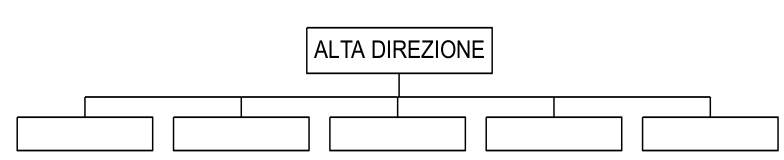
\includegraphics[width=0.5\linewidth]{images/struttura_semplice}
\end{center}

\begin{tabular}{>{\bfseries}l p{90mm}}
	Criterio di raggruppamento: & Funzionale quando esiste
\\
	Meccanismi di coordinamento principali: & Supervisione diretta
	adattamento reciproco, standardizzazione delle capacità
\\
	Imprese giovani di piccole dimensioni
 & \\
	Punti di forza: & Flessibilità \\
	Punti di debolezza: & Conflitto, congestione del vertice \\
\end{tabular}

\subsection{La burocrazia meccanica}
\begin{center}
	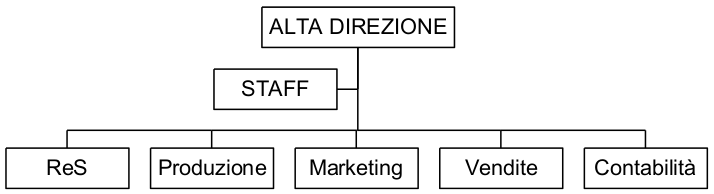
\includegraphics[width=0.5\linewidth]{images/burocrazia_meccanica}
\end{center}

\begin{tabular}{>{\bfseries}l p{90mm}}
	Criterio di divisione del lavoro e raggruppamento: & Specializzazione, funzionale \\
	Meccanismi di coordinamento principali: & Standardizzazione dei
	processi, ruoli di collegamento e comitati
\\
\end{tabular}

Le attività simili (che assolvono la stessa funzione), richiedono le
stesse competenze e utilizzano lo stesso tipo di risorse e di
tecnologie sono raggruppate in un’unica unità organizzativa sotto
un’unica responsabilità.

\proandcons{
	Consente di ottimizzare l’impiego delle risorse umane e tecnologiche
		concentrando risorse simili e ottenendo così economie di scala
		
	Consente inoltre di perseguire una maggiore specializzazione delle competenze
	
	Facilita il controllo gerarchico e la supervisione diretta perché richiede un range
limitato di competenze nei responsabili delle funzioni

}{
	Insoddisfazioni a livello individuale e scarsa condivisione degli obiettivi generali
	
	Può comportare scarso coordinamento tra le diverse funzioni
	
	È solitamente lenta nel reagire ai cambiamenti esterni che richiedono azioni
concertate
	
	Al crescere della dimensione aziendale spesso induce burocratizzazione,
	proliferazione dei livelli gerarchici intermedi, e conseguente rallentamento dei
	processi decisionali

}

\subsection{La burocrazia professionale}
\begin{itemize}
	\item Viene definito \textit{ex ante} il requisito in termini di competenze
	dei lavoratori (ad esempio, uno studio dentistico sceglierà
	laureati in odontoiatria)
	\item I professionisti stessi costituiscono il nucleo operativo
	\item Coordinamento: standardizzazione delle competenze
	decentramento organizzativo e cooperazione reciproca,
	\item Si adatta anche a contesti dinamici, dal momento che si
	suppone che ognuno, grazie al proprio background culturale,
	sappia come comportarsi in caso di eventi imprevisti
\end{itemize}

\subsection{La struttura divisionale}
\begin{center}
	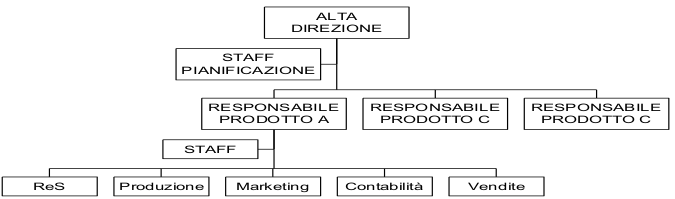
\includegraphics[width=0.5\linewidth]{images/struttura_divisionale}
\end{center}

\begin{tabular}{>{\bfseries}l p{90mm}}
	Criterio di divisione del lavoro: & Prodotto, cliente, area geografica
\\
	Meccanismi di coordinamento principali: & standardizzazione obiettivi \\
	Punti di forza & Velocità di risposta al mercato, possibilità di
	diversificare i prodotti
\\
	Punti di debolezza: & Rinunce alle economie di scala, inefficienza,
	perdita profondità competenze, poca coerenza tra prodotti\\
	Caratteristiche tipiche: & Grandi imprese pluri-prodotto in mercati
	turbolenti e differenziati\\
\end{tabular}

\subsection{Configurazioni organizzative complesse: Adhocrazia}
L'\emph{adhocrazia} rompe il principio di unicità di comando.
\begin{center}
	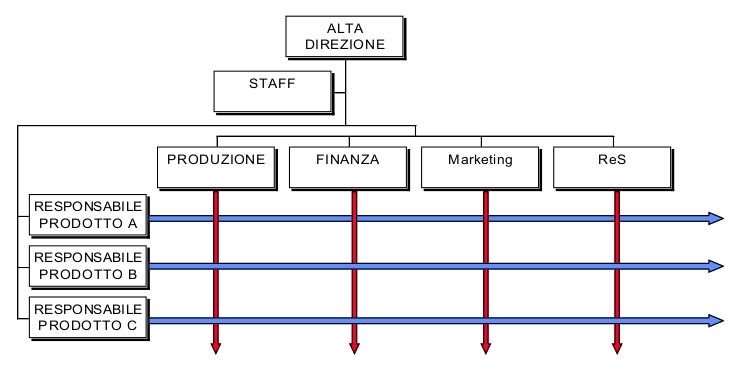
\includegraphics[width=0.5\linewidth]{images/adhocrazia}
\end{center}

\begin{tabular}{>{\bfseries}l p{90mm}}
	Criterio di divisione del lavoro: & Divisionale, funzionale\\
	Meccanismi di coordinamento principali: & Mutuo adattamento, task
	force, struttura a matrice
\\
	Punti di forza: & Velocità di risposta al mercato, possibilità di
	diversificare i prodotti
\\
	Punti di debolezza: & Conflitti, complessità gestionale
 \\
	Caratteristiche tipiche: & Medie imprese pluriprodotto con
	competenze specifiche e operanti in mercati dinamici e complessi \\
\end{tabular}
